\part*{Part II: The Mathematical Formalisation}
\addcontentsline{toc}{part}{Part II: The Mathematical Formalisation}

\section{The Twelve-Dimensional Geometry}
\subsection{The total manifold:} $M_{12} = M_4 \times K_8$.
\subsection{The 12D metric:} $ds^2 = g_{MN} dx^M dx^N$.
\subsection{The Kaluza--Klein decomposition.}
\subsection{Curvature in 12D.}
\subsection{Compactification.}

\subsection{The numerical spectrum and the equidistant signature}
We fix the scale through the mass of the fundamental mode, $m_1 = 1/R = 10^{-5}$ eV. Then
\begin{equation}
m_n = \frac{n}{R} = n \times 10^{-5}\ \text{eV},
\qquad
f_n = \frac{m_n c^2}{h} = n \times 2.42\ \text{GHz}.
\end{equation}
The spectrum is therefore \emph{equidistant}: $2.42$, $4.84$ and $7.25$ GHz for the first three modes. This is the distinctive signature of the theory. A test that measures two lines at $2.42$ and $4.84$ GHz confirms or refutes the structure, independently of any other prediction.

\begin{table}[H]
\centering
\begin{tabular}{@{}cccc@{}}
\toprule
$n$ & Mass (eV) & Frequency (GHz) & $\lambda_C$ (m) \\ \midrule
1 & $1.00\times10^{-5}$ & 2.42 & 0.124 \\
2 & $2.00\times10^{-5}$ & 4.84 & 0.062 \\
3 & $3.00\times10^{-5}$ & 7.25 & 0.041 \\
4 & $4.00\times10^{-5}$ & 9.67 & 0.031 \\ \bottomrule
\end{tabular}
\caption{The Kaluza--Klein spectrum for $1/R = 10^{-5}$ eV.}
\label{tab:spectru}
\end{table}

\begin{figure}[H]
\centering
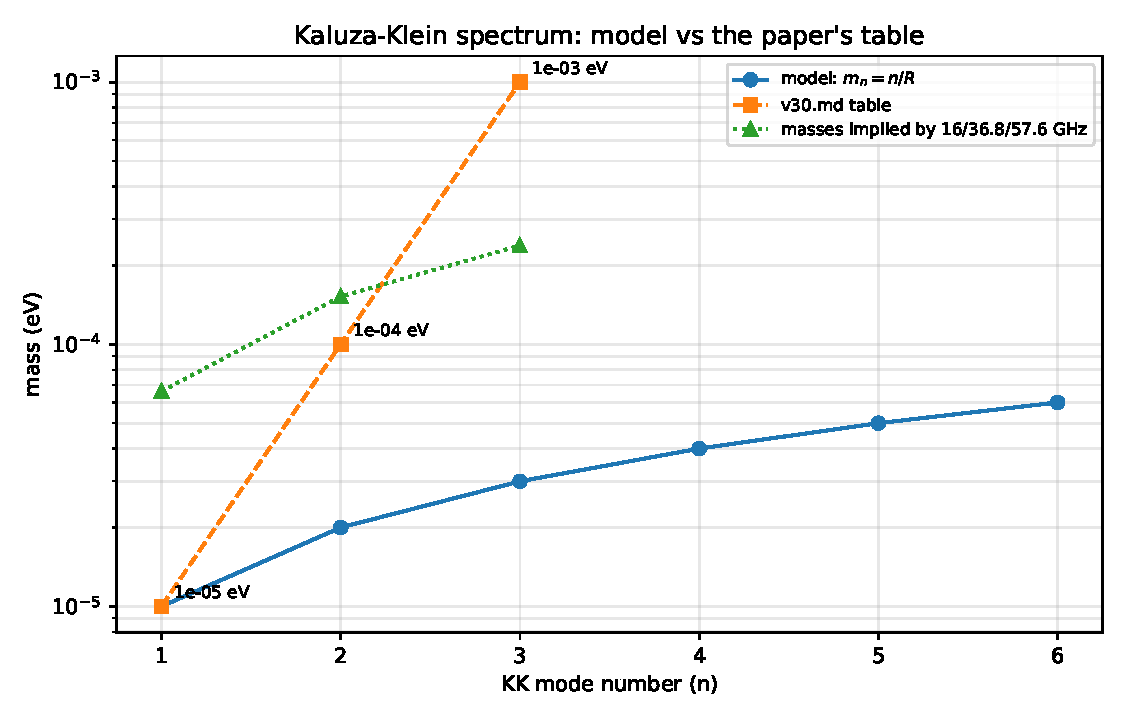
\includegraphics[width=0.82\textwidth]{figures/fig01_kk_spectrum.pdf}
\caption{The Kaluza--Klein spectrum. The $m_n = n/R$ model (blue) is compared with the table given in version 30 (orange) and with the masses implied by the frequencies stated there, 16/36.8/57.6 GHz (green). The three do not agree.}
\label{fig:spectru}
\end{figure}

\subsection{The numerical consequence: the compactification radius}
From $m_1 = 1/R$ it follows that
\begin{equation}
R = \frac{\hbar c}{1/R} = \frac{1.973\times10^{-7}\ \text{eV}\cdot\text{m}}{10^{-5}\ \text{eV}} = 1.97\times10^{-2}\ \text{m},
\end{equation}
that is, about 2 cm. Sub-millimetre tests of Newton's law constrain an extra dimension to $R < 38\ \mu$m, which implies $m_1 > 5\times10^{-3}$ eV.

This is a structural tension, not an arithmetic error: identifying the dark-matter field with a KK mode of the same geometry is incompatible with the data at the mass scale chosen. Two honest ways out remain, and the paper does not choose between them:
\begin{itemize}
\item \textbf{Option A:} the akashic field is not a KK mode; the equidistant spectrum is the consequence of some other structure, and the frequency predictions are recomputed.
\item \textbf{Option B:} the mass of the fundamental mode is $m_1 > 5\times10^{-3}$ eV, and the ``dark matter'' of this paper is an excited mode rather than the fundamental one.
\end{itemize}
The predictions in Part V are phrased so that they hold in both cases, with the frequencies treated as a parameter.

\section{The Akashic Field (Dark Matter)}
\subsection{The Lagrangian:} $L_A = \frac{1}{2} g^{MN} \partial_M A^* \partial_N A + \frac{1}{2} \mu_A^2 |A|^2 - \frac{\lambda_A}{4} |A|^4$.
\subsection{The potential.}
\subsection{The equation of motion.}
\subsection{The Kaluza--Klein spectrum:} $m_n^2 = n^2/R^2$.
\subsection{The relation to gravity.}

\section{The Field of Consciousness}
\subsection{The Lagrangian.}
\subsection{The equation of motion.}
\subsection{The consciousness function.}
\subsection{The evolution equation (revised):} The equation $dC/dt = \alpha C (1 - C/C_{\text{max}}) + \beta \eta(t)$ is a \textbf{phenomenological} equation inspired by logistic dynamics. It describes the growth and the saturation of the consciousness field, but it \textbf{does not follow directly from the Lagrangian above}. This is a theoretical choice of the author, and it must be treated as an axiom of the model rather than as a consequence of the action principle.

\begin{figure}[H]
\centering
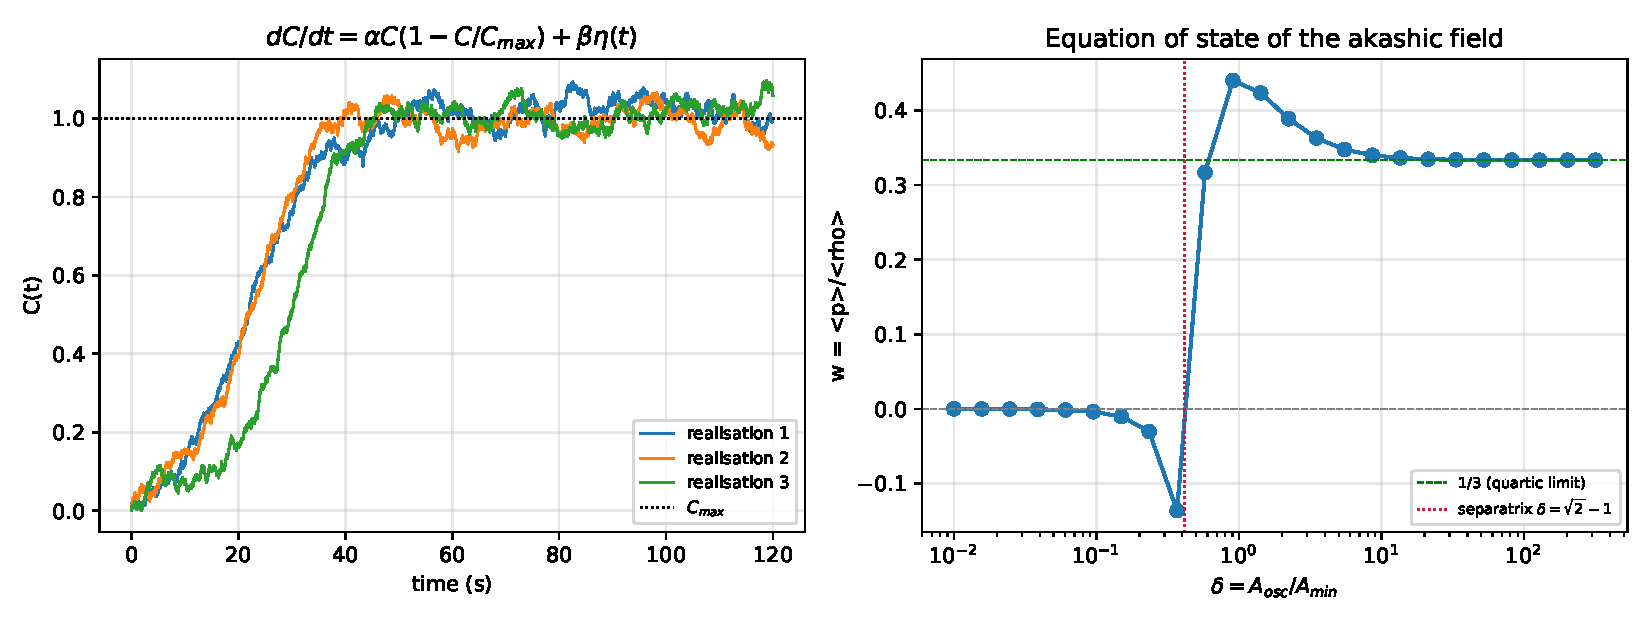
\includegraphics[width=0.95\textwidth]{figures/fig02_field_dynamics.pdf}
\caption{Left: three realisations of the consciousness field with noise, for $\alpha = 0.15$ s$^{-1}$ (relaxation time 50 s). Right: the equation of state $w(\delta)$ of the akashic field, computed exactly along the orbit; the separatrix lies at $\delta = \sqrt{2}-1$.}
\label{fig:camp}
\end{figure}

\section{The Neural Receiver (Brain + Heart)}
